%%% CSE 4316/4317 Senior Design - Test Plan Template
%%% Created 2026 by CDM to follow ISO/IEC/IEEE 29119-3:2021 (Test documentation).
%%% This standard, together with 29119-1/-2/-4, supersedes the withdrawn
%%% IEEE Std 829-2008. The historical IEEE 829 material is retained in the
%%% adjacent "test plan" folder for reference only.

%%%  Preamble
\documentclass[11pt,letterpaper]{article}
\usepackage[margin=1.0in]{geometry}
\usepackage[T1]{fontenc}
\usepackage[bitstream-charter]{mathdesign}
\usepackage[latin1]{inputenc}
\usepackage{amsmath}
\usepackage{xcolor}
\usepackage{cite}
\usepackage{hyphenat}
\usepackage{graphicx}
\usepackage{float}
\usepackage{subfigure}
\usepackage{sectsty}
\usepackage[compact]{titlesec}
\usepackage[tablegrid]{vhistory}
\usepackage{pbox}
\usepackage{longtable}
\allsectionsfont{\color{accentcolor}\scshape\selectfont}

%%% Definitions
\definecolor{accentcolor}{rgb}{0.0,0.0,0.5}
\newcommand{\teamname}{Team Name}
\newcommand{\productname}{Product Name}
\newcommand{\coursename}{CSE 4317: Senior Design II}
\newcommand{\semester}{Spring 2026}
\newcommand{\docname}{Test Plan}
\newcommand{\department}{Department of Computer Science \& Engineering}
\newcommand{\university}{The University of Texas at Arlington}
\newcommand{\authors}{Alan Turing \\ Grace Hopper \\ John Von Neumann \\ Ada Lovelace \\ Charles Babbage}

%%% Headers and footers
\usepackage{fancyhdr}
	\pagestyle{fancy}
\usepackage{lastpage}
	\lhead{}
	\chead{}
	\rhead{}
	\lfoot{\footnotesize \teamname \ - \semester}
	\cfoot{}
	\rfoot{\footnotesize page \thepage\ of \pageref{LastPage}}
	\renewcommand{\headrulewidth}{0.0pt}
	\renewcommand{\footrulewidth}{0.4pt}

\usepackage[runin]{abstract}
\abslabeldelim{\quad}
\setlength{\abstitleskip}{-10pt}
\renewcommand{\abstractname}{}
\renewcommand{\abstracttextfont}{\color{accentcolor} \small \slshape}

\begin{document}

%%% Cover sheet
{\centering \huge \color{accentcolor} \sc \textbf{\department \\ \university} \par}
\vspace{1 in}
{\centering \huge \color{accentcolor} \sc \textbf{\docname \\ \coursename \\ \semester} \par}
\vspace{0.5 in}
\begin{figure}[h!]
	\centering
   	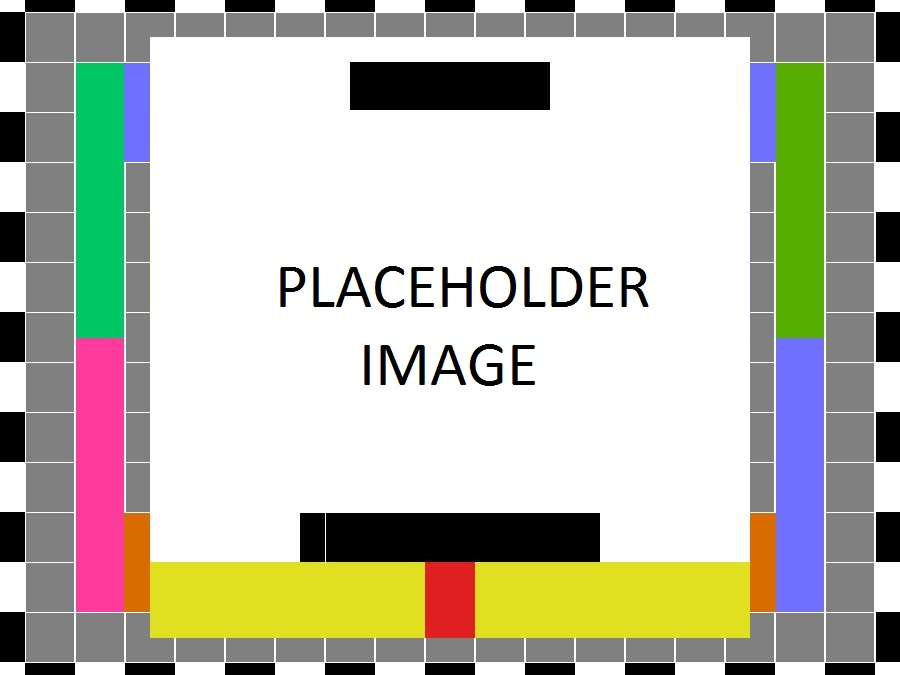
\includegraphics[width=0.60\textwidth]{images/test_image}
\end{figure}
\vspace{0.5 in}
{\centering \huge \color{accentcolor} \sc \textbf{\teamname \\ \productname} \par}
\vspace{0.5 in}
{\centering \large \sc \textbf{\authors} \par}
\newpage

%%% Revision History
\begin{versionhistory}
  	\vhEntry{0.1}{1.15.2026}{GH}{document creation}
  	\vhEntry{0.2}{1.22.2026}{AT|GH}{complete draft}
  	\vhEntry{1.0}{2.01.2026}{AT|GH|CB}{official release}
\end{versionhistory}
\newpage

\setcounter{tocdepth}{2}
\tableofcontents
\newpage
\listoftables
\newpage

%%% NOTE TO STUDENTS (remove before submission):
%%% This Test Plan follows the Test Plan information item of ISO/IEC/IEEE
%%% 29119-3:2021 (Test documentation), part of the 29119 family that supersedes
%%% IEEE Std 829. Test design techniques referenced here are defined in
%%% 29119-4:2021, and testing processes in 29119-2:2021.

\section{Introduction}
This Test Plan defines the testing to be performed for \productname. It is organized as a Test Plan information item per ISO/IEC/IEEE 29119-3:2021 \cite{ISO29119part3}.

\subsection{Purpose}
State the purpose of this document and its intended readers (team, customer, instructor).

\subsection{Scope}
State what testing this plan covers (which items, which test levels) and what it does not.

\subsection{References}
Reference the SRS (source of the requirements under test), the ADS/DDS (source of the design under test), and the applicable parts of ISO/IEC/IEEE 29119 \cite{ISO29119part1, ISO29119part2, ISO29119part3, ISO29119part4}.

\section{Context of Testing}
\subsection{Test Items}
Identify the items to be tested (software builds, firmware, hardware assemblies, integrated system) and their versions/configurations.

\subsection{Features to be Tested}
List the features/requirements in scope for testing. Reference SRS requirement identifiers.

\subsection{Features Not to be Tested}
List features explicitly out of scope for this plan, and why (e.g. deferred/Future requirements).

\subsection{Assumptions \& Constraints}
State the assumptions and constraints affecting testing (environment availability, hardware lead times, access to the customer site, etc.).

\subsection{Test Stakeholders}
Identify who has an interest in the test results (customer, sponsor, instructor, team) and who approves test completion.

\section{Test Risks}
Record the product risks (risks that the product will not meet requirements) and project risks (risks to the testing effort itself) that drive the testing priorities, per ISO/IEC/IEEE 29119-2 \cite{ISO29119part2}.

\begin{table}[H]
\caption{Test risk register (excerpt)}
\begin{center}
    \begin{tabular}{ | p{1.5cm} | p{6cm} | p{2cm} | p{2cm} | p{1.5cm} |}
    \hline
    \textbf{ID} & \textbf{Risk description} & \textbf{Type} & \textbf{Likelihood} & \textbf{Impact} \\ \hline
    R-01 & example product risk & Product & Med & High \\ \hline
    R-02 & example project risk & Project & Low & Med \\ \hline
    \end{tabular}
\end{center}
\end{table}

\section{Test Strategy}
\subsection{Test Sub-Processes (Levels)}
Define the test levels the team will run and the objective of each: unit, integration, system, and acceptance testing. Map each to who performs it and when.

\subsection{Test Design Techniques}
State the techniques used to derive test cases, drawing on ISO/IEC/IEEE 29119-4:2021 \cite{ISO29119part4} --- for example equivalence partitioning, boundary value analysis, decision-table testing, state-transition testing, and, where justified, structural (coverage-based) testing.

\subsection{Test Completion (Entry/Exit) Criteria}
State the entry criteria that must hold before a test level begins and the exit/completion criteria that define ``done'' (e.g. all Critical/High requirements pass; no open Critical defects; target coverage achieved).

\subsection{Suspension \& Resumption Criteria}
State the conditions under which testing is suspended (e.g. a blocking defect) and what must hold to resume.

\subsection{Regression \& Retesting}
Describe how fixed defects are retested and how regression testing is scoped after changes.

\subsection{Metrics}
State the metrics collected (requirements coverage, test pass rate, open-defect counts by severity) and the reporting cadence.

\section{Test Deliverables}
List the documents and artifacts produced: this Test Plan, test case specifications, test data, test scripts, test execution logs/results, defect reports, and the test completion report.

\section{Test Environment \& Tooling}
Describe the hardware, software, network, and data needed to execute the tests, and the tools used (test runners, CI, hardware-in-the-loop rigs, measurement instruments).

\section{Roles, Responsibilities \& Staffing}
Identify who is responsible for test design, execution, and sign-off, and any training required.

\section{Schedule \& Estimates}
Provide the testing schedule aligned to the sprint plan and the effort estimates for the testing tasks.

\section{Test Case Specifications}
Specify each test case using the fields below, adapted from the test case specification of ISO/IEC/IEEE 29119-3 \cite{ISO29119part3}. Repeat per test case.

\subsection{TC-01: [Test Case Title]}
\begin{itemize}
  \item \textbf{Objective:} what this test verifies
  \item \textbf{Traces to:} SRS requirement ID(s) and design element(s)
  \item \textbf{Preconditions:} required state/setup before execution
  \item \textbf{Inputs:} test data / actions
  \item \textbf{Expected results:} the measurable, observable pass condition
  \item \textbf{Test technique:} the 29119-4 technique used to derive the case
  \item \textbf{Priority:} Critical / High / Moderate / Low
\end{itemize}

\section{Requirements Traceability}
Provide a matrix linking every requirement under test to the test case(s) that verify it, closing the traceability chain begun in the SRS and continued through the ADS and DDS.

\begin{table}[H]
\caption{Requirement-to-test-case traceability (excerpt)}
\begin{center}
    \begin{tabular}{ | p{2.5cm} | p{6cm} | p{3cm} |}
    \hline
    \textbf{Req ID} & \textbf{Requirement (abbreviated)} & \textbf{Test case(s)} \\ \hline
    FR-01 & abbreviated requirement text & TC-01, TC-02 \\ \hline
    PE-01 & abbreviated requirement text & TC-05 \\ \hline
    \end{tabular}
\end{center}
\end{table}

%%% References
\bibliographystyle{reference/IEEEtran_custom}
\bibliography{reference/refs}{}

\end{document}
